
\begin{figure*}[h]
     \centering
     \begin{subfigure}[b]{0.45\textwidth}
         \centering
         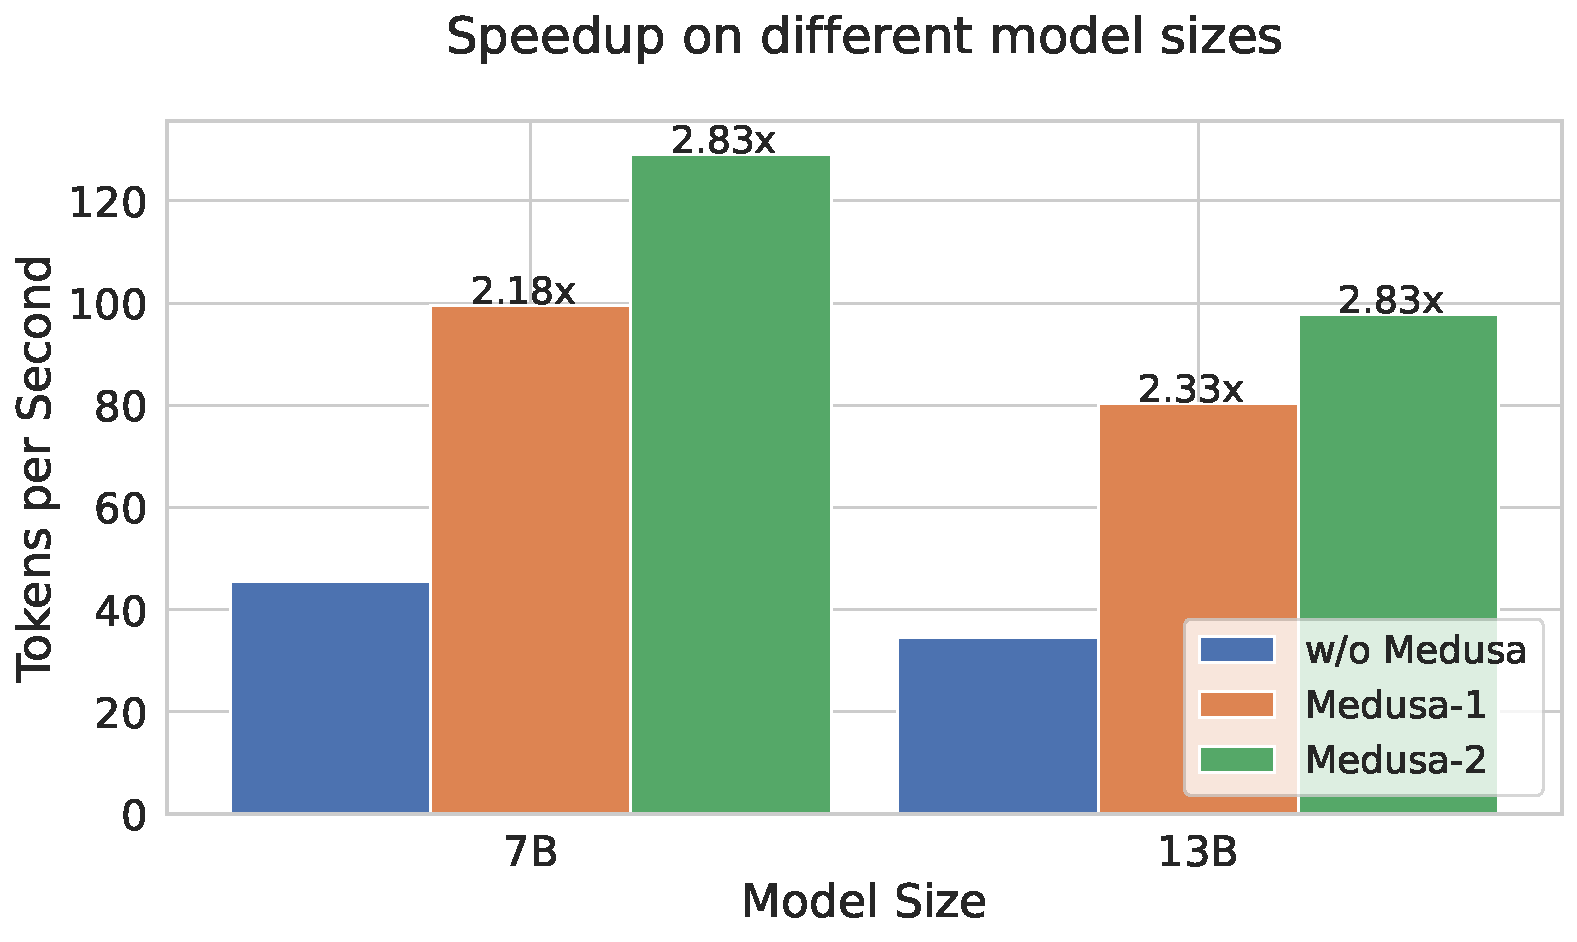
\includegraphics[width=\textwidth]{speedup_model_sizes_wide.pdf}
         \caption{}
         \label{fig:speedup_model_sizes}
     \end{subfigure}
     \begin{subfigure}[b]{0.45\textwidth}
         \centering
         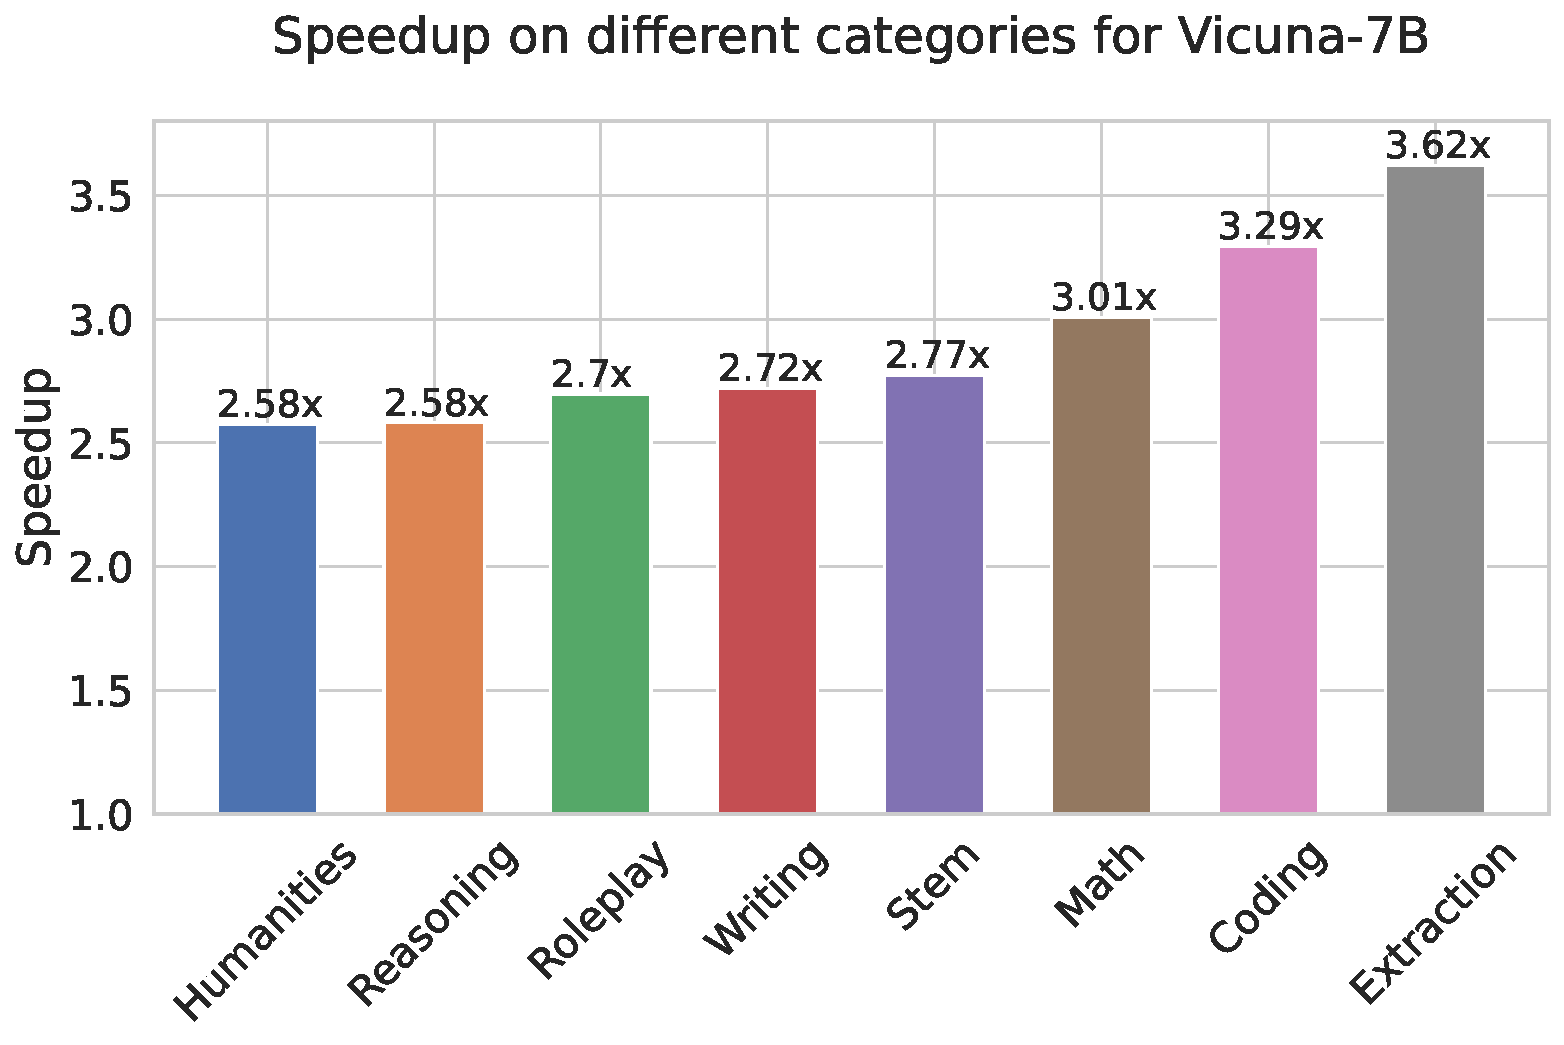
\includegraphics[width=\textwidth]{speedup_per_class_wide.pdf}
         \caption{}
         \label{fig:speedup_per_class}
     \end{subfigure}
        \caption{Left: Speed comparison of baseline, \ours-1 and \ours-2 on Vicuna-7B/13B. \ours-1 achieves more than 2$\times$ wall-time speedup compared to the baseline implementation while \ours-2 further improves the speedup by a significant margin. Right: Detailed speedup performance of Vicuna-7B with \textcolor{black}{\ours-2} on 8 categories from MT-Bench.}
        \label{fig:ablation_tree}
\end{figure*}

\section{Experiments}
In this section, we present experiments to demonstrate the effectiveness of \ours under different settings. First, we evaluate \ours on the Vicuna-7B and 13B models~\citep{vicuna2023} to show the performance of \ours-1 and \ours-2. 
\textcolor{black}{Then, we assess our method using the Vicuna-33B and Zephyr-7B models to demonstrate self-distillation's viability in scenarios where direct access to the fine-tuning recipe is unavailable, as with Vicuna-33B, and in models like Zephyr-7B that employ Reinforcement Learning from Human Feedback (RLHF). The evaluation is conducted on MT-Bench~\citep{zheng2023judging}, a multi-turn, conversational-format benchmark.}
Detailed settings can be found in Appendix~\ref{appendix:experiment_settings}.



\subsection{Case Study: \ours-1 v.s. \ours-2 on Vicuna 7B and 13B}

\textbf{Experimental Setup.}
We use the Vicuna model class~\citep{vicuna2023}, which encompasses chat models of varying sizes (7B, 13B, 33B) that are fine-tuned from the Llama model~\citep{touvron2023llama}. Among them, the 7B and 13B models are trained on the ShareGPT~\citep{sharegpt2023} dataset, while the 33B model is an experimental model and is trained on a private dataset. 
In this section, we use the ShareGPT dataset to train the \ours heads on the 7B and 13B models for $2$ epochs. We use the v1.5 version of Vicuna models, which are fine-tuned from Llama-2 models with sequence length 4096. 


\textbf{Results.}
We collect the results and show them in Fig.~\ref{fig:ablation_tree}. The baseline is the 
\textcolor{black}{default}
Huggingface implementation. In Fig.~\ref{fig:speedup_model_sizes}, we can see that for the 7B models, \ours-1 and \ours-2 configurations lead to a significant increase in speed, measuring in tokens processed per second. \ours-1 shows a 2.18$\times$ speedup, while \ours-2 further improves this to a 2.83$\times$.
When applied to the larger 13B model, \ours-1 results in a 2.33$\times$ speed increase, while \ours-2 maintains a similar performance gain of 2.83$\times$ over the baseline.
We also plot the speedup per category for \ours-2 Vicuna-7B model. 
We observe that the coding category benefits from a 3.29$\times$ speedup, suggesting that \ours is particularly effective for tasks in this domain. This points to a significant potential for optimizing coding LLMs, which are widely used in software development and other programming-related tasks. 
The ``Extraction'' category shows the highest speedup at 3.62$\times$, indicating that this task is highly optimized by the \ours.
Overall, the results suggest that the \ours significantly enhances inference speed across different model sizes and tasks.


\subsection{Case Study: Training with Self-Distillation on Vicuna-33B and Zephyr-7B}
\textbf{Experimental Setup.}
In this case study, we focus on the cases where self-distillation is needed. We use the Vicuna-33B model~\citep{vicuna2023} and the Zephyr-7B model~\citep{tunstall2023zephyr} as examples. Following the procedure described in Section~\ref{sec:self_distillation}, we first generate the datasets with some seed prompts. We use ShareGPT~\citep{sharegpt2023} and UltraChat~\citep{ding2023enhancing} as the seed datasets and collect a dataset at about $100k$ samples for both cases. Interestingly, we find that the Zephyr model can continue to generate multiple rounds of conversation with a single prompt, which makes it easy to collect a large dataset. 
For Vicuna-33B, we generate the multi-turn conversations by iteratively feeding the prompts from each multi-turn seed conversation \textcolor{black}{using random sampling with temperature 0.3}. Both models are trained with sequence length $2048$ and batch size $128$. 
\begin{table}[h]
\centering
\scriptsize
\begin{tabular}{@{}lllll@{}}
\toprule
Model Name & Vicuna-7B & Zephyr-7B & Vicuna-13B & Vicuna-33B \\ \midrule
Acc. rate   & 3.47      & 3.14      & 3.51       & 3.01       \\ 
Overhead   & 1.22      & 1.18      & 1.23       & 1.27       \\ 
Quality    & 6.18 (+0.01) & 7.25 (-0.07) & 6.43 (-0.14) & 7.18 (+0.05) \\ \midrule
$S_{\textnormal{SpecDecoding}}$ & 1.47 & - & 1.56 & 1.60 \\
$S_\ours$ & 2.83 & 2.66 & 2.83 & 2.35\\\bottomrule
\end{tabular}
\caption{Comparison of various \ours-2 models. 
\textcolor{black}{The first section reports the details of \ours-2, including accelerate rate, overhead, and quality that denoted the average scores on the MT-Bench \textcolor{black}{compared to the original models}. The second section lists the speedup ($S$) of SpecDecoding and \ours, respectively.}
}


\label{tab:all_model_results}
\end{table}

\begin{figure*}[ht]
     \centering
     \begin{subfigure}[b]{0.45\textwidth}
         \centering
         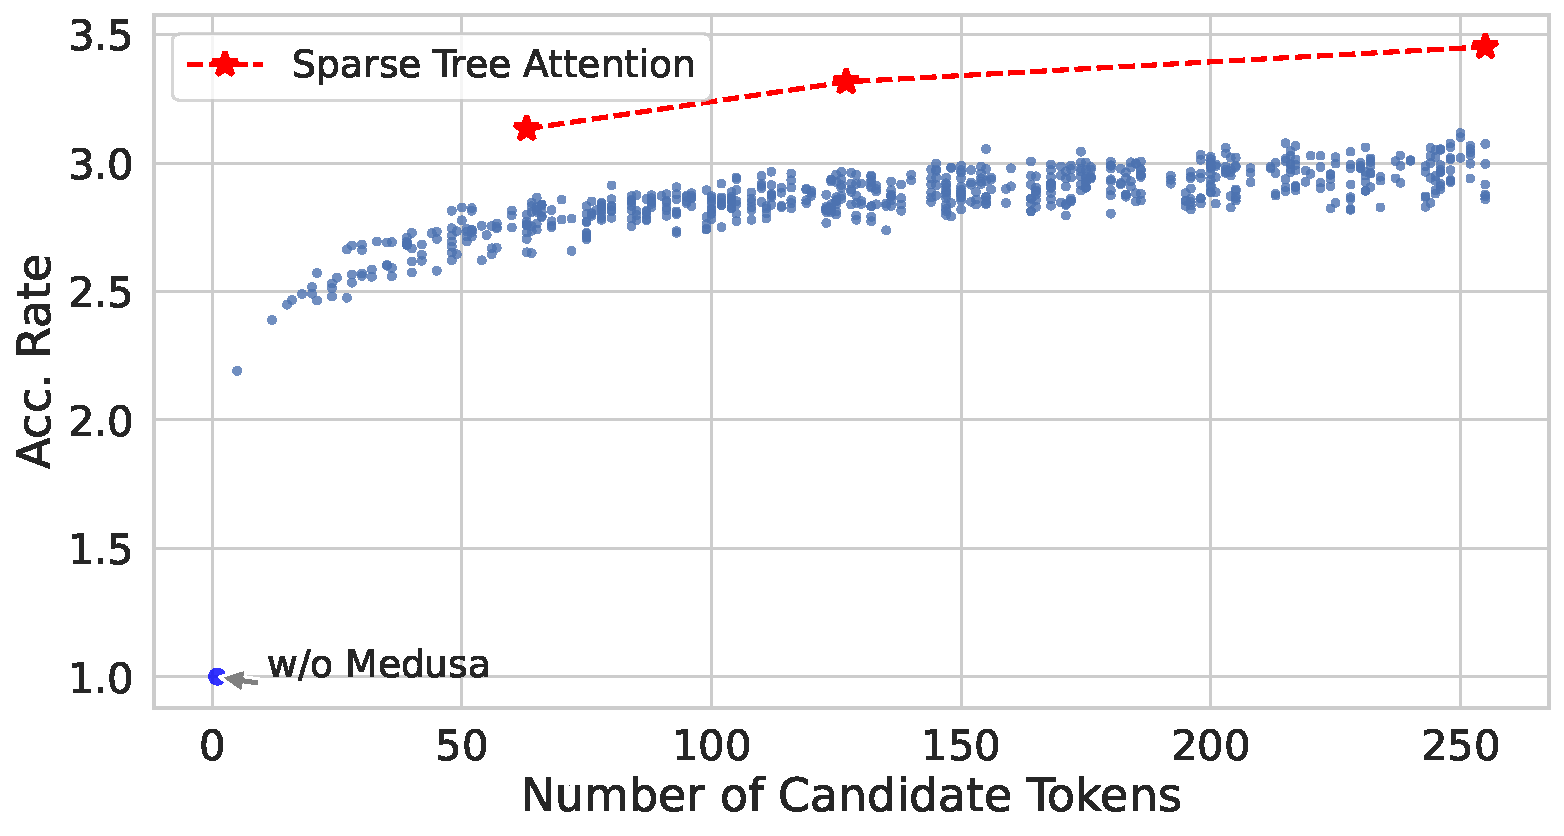
\includegraphics[width=\textwidth]{sparse_acc.pdf}
         \caption{}
         \label{fig:sparse_acc}
     \end{subfigure}
     \begin{subfigure}[b]{0.45\textwidth}
         \centering
         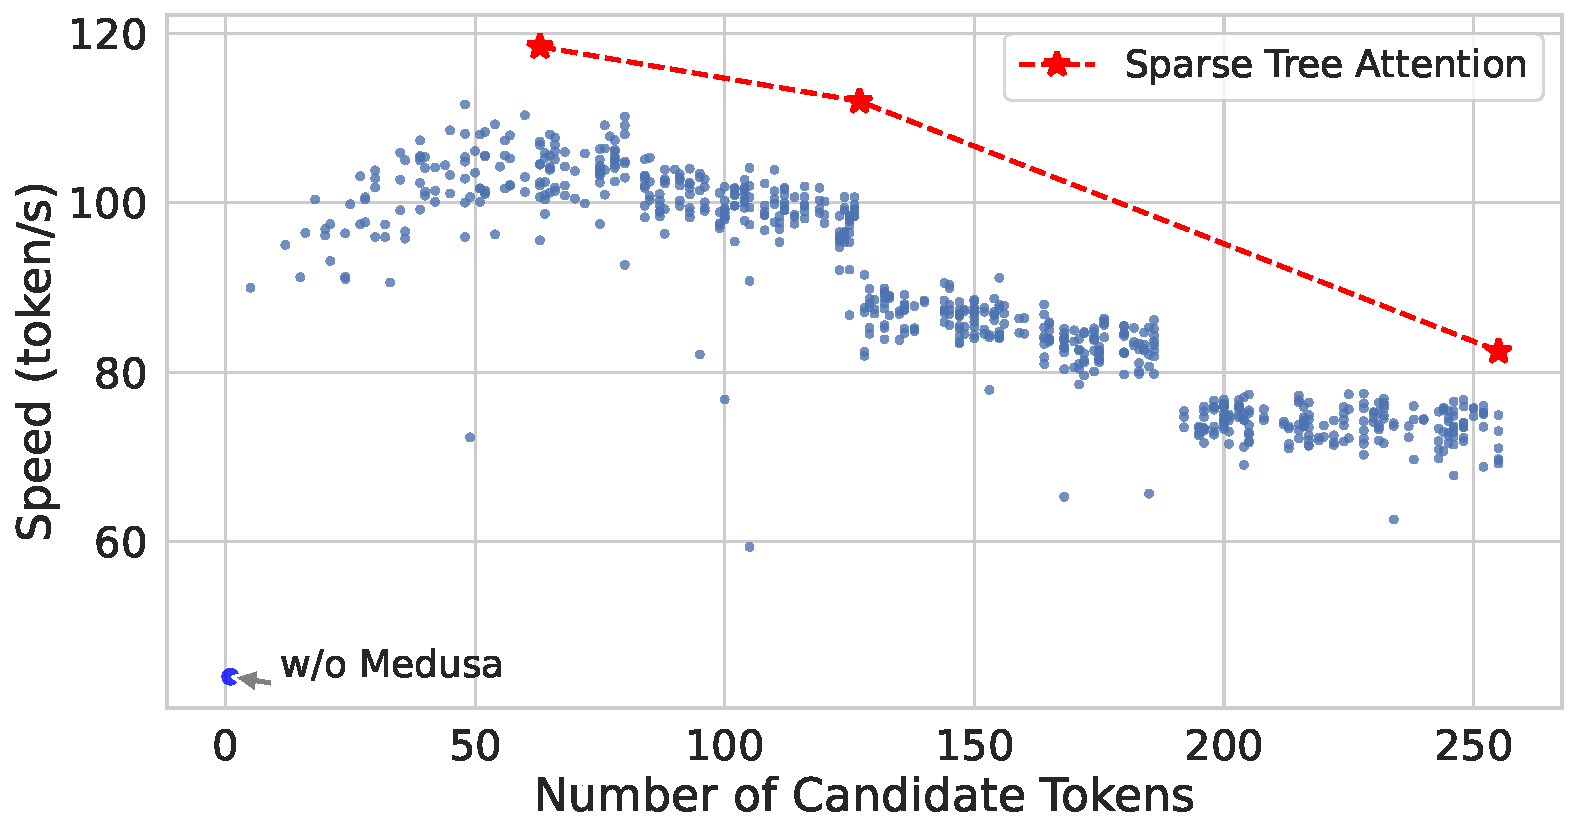
\includegraphics[width=\textwidth]{sparse_speed.pdf}
         \caption{}
         \label{fig:sparse_speed}
     \end{subfigure}
\vspace{-4mm}
        \caption{Effectiveness of numbers of candidate tokens for decoding introduced by trees (default number of candidate token for decoding is 1 when using KV cache). Left: The acceleration rate for randomly sampled dense tree settings (blue dots) and optimized sparse tree settings (red stars). Right: The speed (tokens/s) for both settings. The trend lines indicate that while the \textcolor{black}{acceleration} rate remains relatively stable for sparse trees, there is a notable decrease in speed as the candidate tokens increases.}
        \label{fig:sparse_tree_ablation}
\end{figure*}

\textbf{Results.}
Table~\ref{tab:all_model_results} complements these findings by comparing various \ours-2 models in terms of their acceleration rate, overhead, and quality on MT-Bench \textcolor{black}{with GPT-4 acting as the evaluator to assign performance scores ranging from 0 to 10. We report the quality differences of \ours compared to the original model. 
} 
Notably, while the \ours-2 Vicuna-33B model shows a lower acceleration rate, it maintains a comparable quality. We hypothesize that this is due to a mismatch between the hidden training dataset and the dataset we used for self-distillation. \textcolor{black}{Hence, the model's generation quality can be well aligned by self-distillation while \ours heads learn distribution from the self-distillation that potentially shifts from the training set.}
In our study, we also applied speculative decoding~\citep{chen2023accelerating,leviathan2022fast} to the Vicuna lineup using open-source draft models (details can be found
in Appendix~\ref{appendix:spec}).


These results underscore the complex interplay between speed and performance when scaling up model sizes and applying self-distillation techniques. The findings also highlight the potential of the \ours-2 configuration to boost efficiency in processing while carefully preserving the quality of the model's outputs, suggesting a promising direction for co-optimizing LLMs with \ours heads.




\subsection{Ablation Study}
\subsubsection{Configuration of Tree Attention}~\label{section:config of tree}
The study of tree attention is conducted on the writing and roleplay categories from the MT-Bench dataset using \ours-2 Vicuna-7B. We target to depict tree attention's motivation and its performance. 

Fig.~\ref{fig:sparse_acc} compares the acceleration rate of randomly sampled dense tree configurations (Section.~\ref{sec:tree_attention}, depicted by blue dots) against optimized sparse tree settings (Section.~\ref{sec:optimized_tree_construction}, shown with red stars). The sparse tree configuration with 64 nodes shows a better acceleration rate than the dense tree settings with 256 nodes.
The decline in speed in Fig.~\ref{fig:sparse_speed} is attributed to the increased overhead introduced by the \textcolor{black}{compute-bound. While a more complex tree can improve acceleration, it does so at the cost of speed due to intensive matrix multiplications for linear layers and self-attention. The acceleration rate increase follows a logarithmic trend and slows down when the tree size grows as shown in Fig.~\ref{fig:sparse_acc}. However, the initial gains are substantial, allowing Medusa to achieve significant speedups. If the acceleration increase is less than the overhead, it will slow down overall performance.} For detailed study, please refer to Appendix~\ref{sec:roofline}.

\begin{figure}[H]
    \centering
    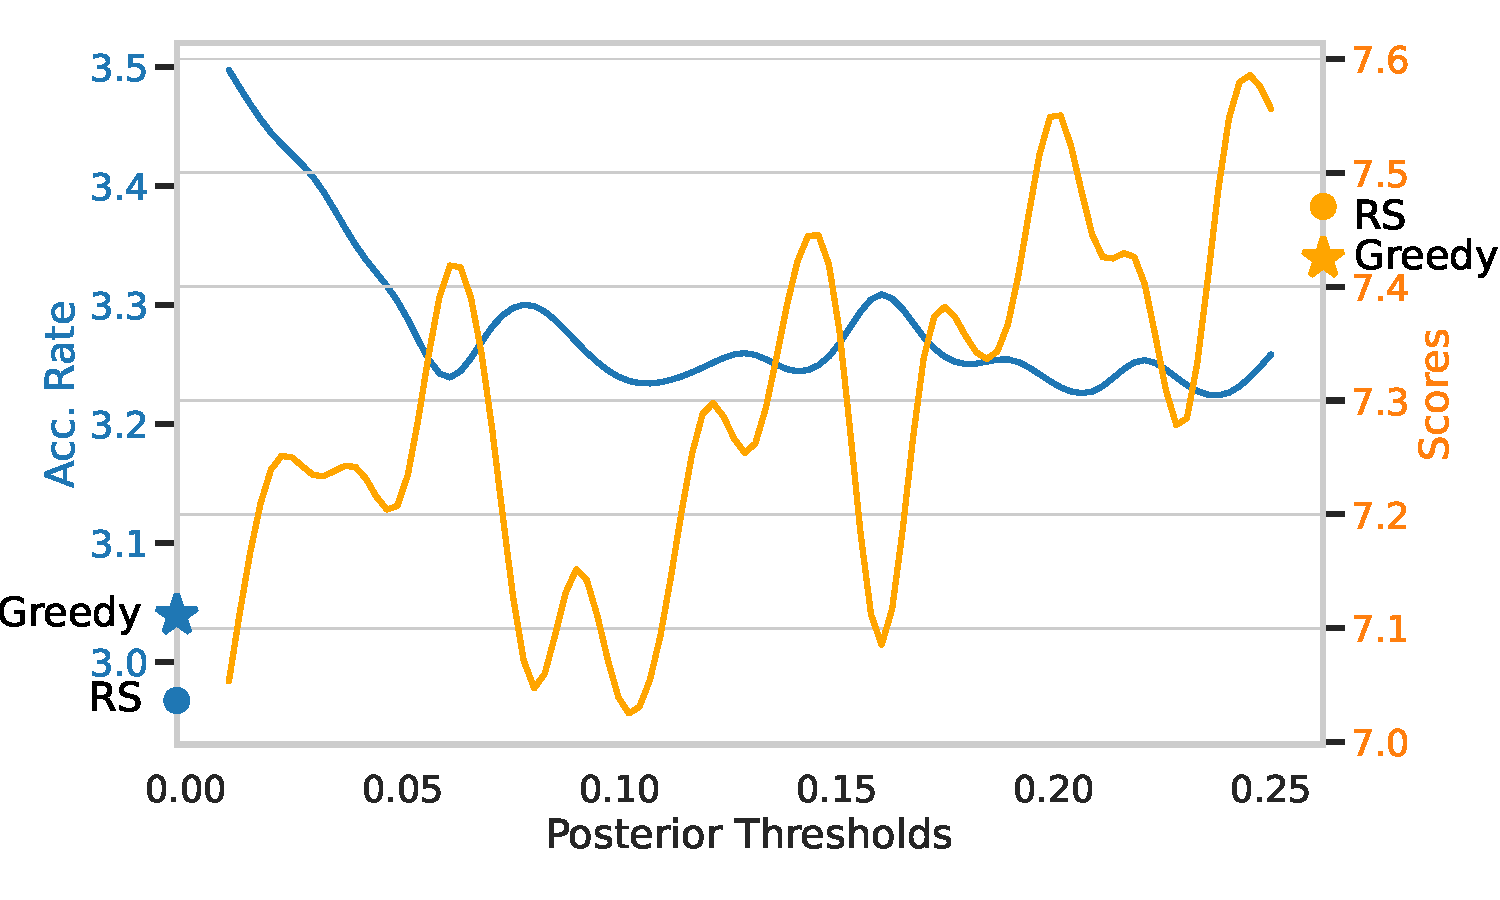
\includegraphics[width=0.45\textwidth]{threshold_ablation_wide.pdf}
    \caption{ Performance comparison of \ours using proposed typical sampling. The model is fully fine-tuned from Vicuna-7B. The plot illustrates the acceleration rate and average scores on the writing and roleplay (MT-Bench) with a fixed temperature of 0.7 for 3 different settings: \textcolor{black}{greedy sampling and random sampling (RS) plotted as the star and the dot, and typical sampling curves under different thresholds.}}
    \label{fig:threshold_ablation}
\end{figure}

\subsubsection{Thresholds of Typical Acceptance}
The thresholds of typical acceptance are studied on the writing and roleplay categories from the MT-Bench dataset~\citep{zheng2023judging} using \ours-2 Vicuna 7B. 
Utilizing the Vicuna 7B model, we aligned our methodology with the approach delineated by
~\cite{hewitt2022truncation} setting the $\alpha = \sqrt{\epsilon}$. 
Fig.~\ref{fig:threshold_ablation} presents a comparative analysis of our model's performance across various sampling settings.
These settings range from a threshold $\epsilon$ starting at 0.01 and incrementally increasing to 0.25 in steps of 0.01. Our observations indicate a discernible trade-off: as $\epsilon$ increases, there is an elevation in quality at the expense of a reduced acceleration rate. Furthermore, for tasks demanding creativity, it is noted that the default random sampling surpasses greedy sampling in performance, and the proposed typical sampling is comparable with random sampling when $\epsilon$ increases.




\begin{table}[h!]
\centering
\scriptsize
\begin{tabular}{@{}lcccccc@{}}
\toprule
               & Baseline & Direct Fine-tuning &  \ours-1 & \ours-2 \\ \midrule
Quality        & 6.17        & 5.925            & 6.23        & 6.18        \\ 
Speedup       & N/A                & N/A            & 2.18        & 2.83        \\
\bottomrule
\end{tabular}

\caption{Comparison of Different Settings of Vicuna-7B. Quality is obtained by evaluating models on MT-Bench \textcolor{black}{using GPT-4 as the judge (higher the better)}.}
\label{tab:7b settings}
\end{table}


\subsubsection{Effectiveness of Two-stage Fine-tuning}

\textcolor{black}{
Table~\ref{tab:7b settings} shows the performance differences between various fine-tuning strategies for the Vicuna-7B model. \ours-1, which fine-tunes only the \ours heads, achieves a 2.18x speedup without compromising generation quality. \ours-2, which employs two-stage fine-tuning (Section~\ref{sec:joint_training}), maintains generation quality and provides greater speedup (2.83x) compared to \ours-1. In contrast, direct fine-tuning the model with the \ours heads results in degraded generation quality. 
}
The findings indicate that implementing our \ours-2 for fine-tuning maintains the model's quality and concurrently improves the speedup versus \ours-1.

\begin{table}[h]
    \centering
    \caption{Impact of Techniques on Speedup}
    \begin{tabular}{lc}
    \toprule
    Technique & Speedup \\ \midrule
    Medusa-1 heads without tree attention & $\sim$1.5x \\
    Adding tree attention & $\sim$1.9x \\
    Using optimized tree configuration & $\sim$2.2x \\
    Training heads with Medusa-2 & $\sim$2.8x \\ \bottomrule
    \end{tabular}
    \label{tab:impact_of_tech}
\end{table}

\section{Discussion}
In conclusion, \ours enhances LLM inference speed by 2.3-2.8 times by equipping models with additional predictive decoding heads, allowing for generating multiple tokens simultaneously and bypassing the sequential decoding limitation. Key advantages of \ours include its simplicity, parameter efficiency, and ease of integration into existing systems.
\ours avoids the need for specialized draft models. The typical acceptance scheme removes complications from rejection sampling while providing reasonable outputs. Our approach including two efficient training procedures, ensures high-quality output across various models and prompt types. We summarize the development of each technique and their impact on the speedup in Table~\ref{tab:impact_of_tech}.

In the paper, we focus on the setting with batch size 1 for simplicity. Yet, we want to emphasize that the ideas presented in our paper can be generalized to larger batch-size settings, which are now supported by libraries like TensorRT and Huggingface TGI following our paper. 

\section*{Acknowledgements}
We extend our heartfelt gratitude to several individuals whose contributions were invaluable to this project:
\begin{itemize}
    \item Zhuohan Li, for his invaluable insights on LLM serving. If you haven't already, do check out Zhuohan's vLLM project—it's nothing short of impressive.
    \item Shaojie Bai, for engaging in crucial discussions that helped shape the early phases of this work.
    \item Denny Zhou, for introducing the truncation sampling scheme to Tianle and encouraging Tianle to explore the area of LLM serving.
    \item Yanping Huang, for pointing out the memory-bandwidth-bound challenges associated with LLM serving to Tianle.
    \item Lianmin Zheng, for clarifying the different training recipes used in different sizes of Vicuna models.
\end{itemize}
\textcolor{black}{Jason D. Lee} acknowledges the support of the NSF CCF 2002272, NSF IIS 2107304, and NSF CAREER Award 2144994. \textcolor{black}{Deming Chen acknowledges the support from the AMD Center of Excellence at UIUC.}

\section*{Impact Statement}
The introduction of \ours, an innovative method to improve the inference speed of Large Language Models (LLMs), presents a range of broader implications for society, technology, and ethics. This section explores these implications in detail.

\subsection*{Societal and Technological Implications
}
\begin{itemize}
    \item \textbf{Accessibility and Democratization of AI}: By significantly enhancing the efficiency of LLMs, \ours makes advanced AI technologies more accessible to a wider range of users and organizations. Democratization can spur innovation across various sectors, including education, healthcare, and entertainment, potentially leading to breakthroughs that benefit society at large.
    \item \textbf{Environmental Impact}: The acceleration for LLM inference due to \ours could lead to decreased energy consumption and a smaller carbon footprint. This aligns with the growing need for sustainable AI practices, contributing to environmental conservation efforts.
    \item \textbf{Economic Implications}: The increased efficiency brought about by \ours may lower the cost barrier to deploying state-of-the-art AI models, enabling small and medium-sized enterprises to leverage advanced AI capabilities. This could stimulate economic growth, foster competition, and drive technological innovation.
    \end{itemize}
\subsection*{Ethical Considerations}
\begin{itemize}
    \item \textbf{Bias and Fairness}: While \ours aims to improve LLM efficiency, it inherits the ethical considerations of its backbone models, including issues related to bias and fairness. The method's ability to maintain generation quality necessitates investigation to ensure that the models do not perpetuate or amplify existing biases.

 \item \textbf{Transparency and Accountability}: The complexity of \ours, particularly with its tree-based attention mechanism and multiple decoding heads, may pose challenges in terms of model interpretability. Ensuring transparency in how decisions are made and maintaining accountability for those decisions are crucial for building trust in AI systems.

\item \textbf{Security and Privacy}: The accelerated capabilities of LLMs augmented by \ours could potentially be exploited for malicious purposes, such as generating disinformation at scale or automating cyber-attacks. It is imperative to develop and enforce ethical guidelines and security measures to prevent misuse.

\end{itemize}













